\subsection{Enhanced Helium Hermeticity in Micro-fabricated Vapor Cells}
Helium plays a critical role in the operation of various atomic sensors, serving
primarily as a working medium or buffer gas in high-sensitivity applications
(e.g., magnetoencephalography \cite{labyt2019}). However, due to its extremely
small atomic radius, helium exhibits one of the highest permeation rates
through glass walls compared to other gases and alkali metals typically
confined within micro-electromechanical systems (MEMS) vapor cells.
\\\\
For high-precision applications where long-term cell hermeticity is paramount,
aluminum oxide (Al$_{2}$O$_{3}$, or alumina) has been identified as a highly
effective barrier \cite{carle2023, Dellis2016}. Researchers have found that
utilizing aluminosilicate glass---a glass matrix enriched with
Al$_{2}$O$_{3}$---or depositing thin Al$_{2}$O$_{3}$ coatings directly onto
standard glass cells significantly mitigates helium diffusion. 
\\\\
As illustrated in Figure \ref{fig:He}, the permeability constant ($K$) of
aluminosilicate glass is between two and three orders of magnitude lower than
that of conventional borosilicate glass. Furthermore, applying an Al$_{2}$O$_{3}$
coating to borosilicate cells can independently reduce helium permeability by one
to two orders of magnitude. Synergistically combining an aluminosilicate glass
substrate with the aforementioned Al$_{2}$O$_{3}$ coating yields the best results,
achieving ultra-low permeabilities on the order of
$10^{-22}\text{ m}^{2}\text{s}^{-1}\text{Pa}^{-1}$.
\begin{figure}[h]
    \centering
    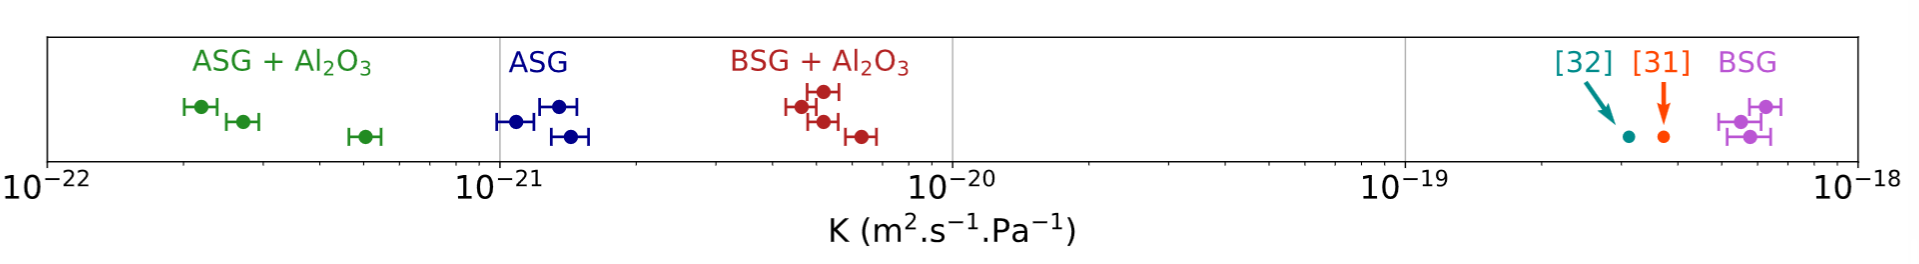
\includegraphics[width=\textwidth]{Images/He.png} 
    \caption{Comparison of the permeability constant $K$ across uncoated borofloat,
     uncoated aluminosilicate, Al$_{2}$O$_{3}$-coated borofloat, and Al$_{2}$O$_{3}$-coated
      aluminosilicate glasses. From \cite{carle2023}.}
    \label{fig:He}
\end{figure}